\documentclass[a4paper,chapter,kosection,atbegshi,hidelinks,itemph]{oblivoir}
\usepackage[dbl4x6]{fapapersize}
\usepackage{amsmath,amssymb,amsfonts,mdframed,enumitem,graphicx,wrapfig,xcolor}
\graphicspath{{./IMG/}}
\setlist{nosep}

\renewcommand\chaptername{강}

\makepagestyle{hf}
\makeevenhead{hf}{\thepage}{}{\itshape\leftmark}
\makeoddhead{hf}{}{}{\thepage}
\makeevenfoot{hf}{}{}{}
\makeoddfoot{hf}{}{}{}
\makepsmarks{hf}{%
\createmark{chapter}{left}{nonumber}{}{}}

\begin{document}
\title{양자정보학 개론\thanks{원문: \url{https://www.scottaaronson.com/qclec.pdf}}}
\author{
    스콧 애론슨\thanks{코리 오스트로브와 파울로 알브스의 큰 도움을 받았다.}, 
    2018년 가을\\
    번역: 김태원
}
\date{\today}
\newpage
\maketitle\thispagestyle{empty}\newpage

\tableofcontents\pagestyle{plain}

\chapter{강의 개요 및 확장 처치-튜링 논제}
\begin{itemize}[label=\(\blacktriangleright\)]
    \item 양자정보학은 천성이 간학문적인 분야다. (물리학, 전산학, 수학, 공학, 철학)
    \item 양자정보학은 단지 유용한 장치나 알고리즘의 발명만이 아니라 양자역학적 작용의 명료화에 관한 것이기도 하다.
    \begin{itemize}
        \item 양자역학으로 할 수 있느냐 없느냐는 물음을 던지기 위한 것이자
        \item 양자역학 자체의 본성에 대한 더 나은 이해를 독려하기 위한 것이다.
    \end{itemize}
    \item 애론슨 교수는 양자정보학 연구의 이론적인 극단에 헌신한다.
    \item 이론가들은 실험가들이 만드는 것을 알리고 이는 다시 이론가들의 질문에 영향을 미친다.
\end{itemize}\hfill\break
오늘은 물리적 세계에 관해 ``자명한" 진술들을 명시한다.
그런 다음 양자역학이 이들 진술 가운데 몇몇만 놔두고 나머지는 뒤엎어 버리는 광경을
목도할 텐데, 이들 진술 간의 차이란 종종 아주 미묘하다!
우선...\hfill\break

\begin{description}[leftmargin=0cm]
    \item[\textbf{확률}\;] 
        $(P\in[0,1])$는 세상의 불확실성을 나타내는 표준적인 방법이다. 
        확률은 아래 같은 일련의 공리를 따라야 한다.
        \begin{itemize}[label=$\blacktriangleright$]
            \item  상호배타적이며 포괄적인 사건{\footnotesize mutually exclusive
            exhaustive events} $n$개의 집합에 대해  
                확률들의 합은 $P_1+P_2+\cdots+P_n=1$을 만족한다.
            \item 임의의 사건에 대한 확률은 $P_i\geq0$을 만족한다.
        \end{itemize}
        \begin{align*}\bullet\\\bullet\\\bullet\end{align*}
\end{description}

\newpage\pagestyle{hf}

\hfill\parbox[t]{9cm}{\textcolor{gray}{\slshape``확률은 전부 우리 손 안에 있다"는
관점이 존재한다. 우주에 관해 전부 (요컨대 태양계 속 모든 원자의 
위치/속도를) 안다면, 방정식들을 처리해서 뭐가 일어나는지 아닌지
보기만 하면 그만이라는 뜻이다.}}\break

\begin{wrapfigure}{r}{0.35\textwidth}
    \centering
    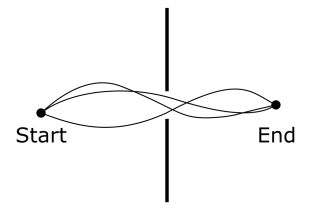
\includegraphics[width=0.35\textwidth]{iqis1_001}
\end{wrapfigure}

\hfill

슬릿 하나를 지닌 장벽이 두 점을 구분하고 있다고 하자. 우리는 입자가 한 점에서 다른
점으로 이동하는 확률을 측정하고자 한다. 경로를 늘리면 (다시 말해 또 다른 슬릿을 
개방하면) 다른 쪽에 도달할 가능성이 증가, 아니 적어도 감소하지는 않을 것은
분명하다. 확률이 \textbf{단조}{\footnotesize monotone}라는 말로 이런 성질을
가리킬 수 있다.

\hfill
\begin{description}[leftmargin=0cm]
    \item[국소성{\footnotesize Locality}] 
        사물은 우주를 가로지를 때 오직 특정 속도로 전파할 수 있을 따름이다.
        공간의 조각 하나의 상태를 갱신할 때는 그 부분을 둘러싸는 주변부에
        대한 지식만이 요구되어야 할 것이다. 이에 적절한 모델은 콘웨이의
        생명게임{\footnotesize Game Of Life}이다. 계{\footnotesize system}에 
        일으키는 변화는 계에 영향을 미칠 수 있다. 하지만 각 칸이 상호작용하는
        대상은 가장 가까운 주변부 뿐이다. 그리하여 변화는 오직 특정 속도로
        전파한다.
\end{description}

\begin{wrapfigure}{l}{0.33\textwidth}
    \centering
    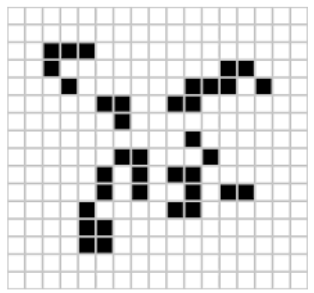
\includegraphics[width=0.33\textwidth]{iqis1_002}
\end{wrapfigure}

\hfill

국소성은 물리학에서 자연스럽게 모습을 드러낸다. 아인슈타인의 특수상대성이론
덕분인데 이는 어떤 신호도 빛의 (유한한) 속력보다 빠르게 전파할 수 없다는
암시를 지니는 원리다. 이 간단한 원리는 다수의 물리 현상을 설명할 수 있다. 
특수상대성이론에 따르면 광속보다 빠르게 이동하는 것들 전부 다 어떤 관찰자의 
관점으로는 실상 시간을 역행하고 있다.\break

\begin{description}[leftmargin=0cm]
    \item[국소적 실재론{\footnotesize Local Realism}] 멀리 떨어진 사건에 대해 
        이루어지는 지식의 갱신을 전부 무작위 변수의 상관관계로 설명할 수 있다는
        원리다. 당신은 오스틴, 친구는 샌프란시스코에 있고 둘 다 동일한 신문을
        구독한다고 하자. 이제 당신은 아침에 신문을 펼쳤다. 그러자 당신의 지식은
        즉각 붕괴한다. 바로 샌프란시스코 친구가 지니는 신문의 헤드라인에 관한
        지식이었다. 붕괴의 자리에 당신이 지금 손에 쥔 신문의 헤드라인이 들어선다.
        아침에 신문을 집기 전이라면 당신이 지니는 지식은 확률 분포로 가장 잘
        서술될 테다. 하지만 그 결과가 완벽하게 상호연관되어 있기에 신문 헤드라인
        학습의 바로 그 순간 즉각 친구의 신문도 동일한 헤드라인을 지닌다고 안다.
        \end{description}

\newpage
\hfill\parbox[t]{9cm}{어떤 }
\end{document}
